\documentclass[10pt,fleqn]{article} % Default font size and left-justified equations
\usepackage[%
    pdftitle={Energétique},
    pdfauthor={Xavier Pessoles}]{hyperref}

    
\input{style/new_style}
\input{style/macros_SII}
\usepackage{multicol}
\usepackage{siunitx}
%\usepackage{picins}
\fichetrue
%\fichefalse

\proftrue

\proffalse

\tdtrue
%\tdfalse

\courstrue
\coursfalse


\def\classe{\textsf{PT}}
\def\xxnumpartie{}%Cycle --}
\def\xxpartie{ }

\def\xxnumchapitre{}%Chapitre -- \vspace{.2cm}}
\def\xxchapitre{\hspace{.12cm} }

\def\discipline{Sciences \\Industrielles de \\ l'Ingénieur}
\def\xxtete{Sciences Industrielles de l'Ingénieur}


  
\def\xxposongletx{2}
\def\xxposonglettext{1.45}
\def\xxposonglety{20}
%\def\xxonglet{Part. 1 -- Ch. 3}
\def\xxonglet{\textsf{}}%Cycle 05}}

\def\xxactivite{Colle 01}
\def\xxauteur{\textsl{Xavier Pessoles}}


\def\xxtitreexo{Siège motorisé}
\def\xxsourceexo{\hspace{.2cm} \footnotesize{BTS CPI 2018}}


\def\xxcompetences{%
\vspace{-.5cm}
\footnotesize{
\textsl{%
\textbf{Savoirs et compétences :}\\
\vspace{-.2cm}
%\begin{itemize}[label=\ding{112},font=\color{ocre}] 
%\item Mod2.C18.SF1 : Déterminer l’énergie cinétique d’un solide, ou d’un ensemble de solides, dans son mouvement par rapport à un autre solide.
%\item Res1.C1.SF1 : Proposer une démarche permettant la détermination de la loi de mouvement.
%\item Mod1.C5.SF2 : Déterminer la puissance des actions mécaniques extérieures à un solide ou à un ensemble de solides, dans son mouvement rapport à un autre solide.
%\item Mod1.C5.SF3 : Déterminer la puissance des actions mécaniques intérieures à un ensemble de solides.
%\end{itemize}
}}}

\def\xxfigures{
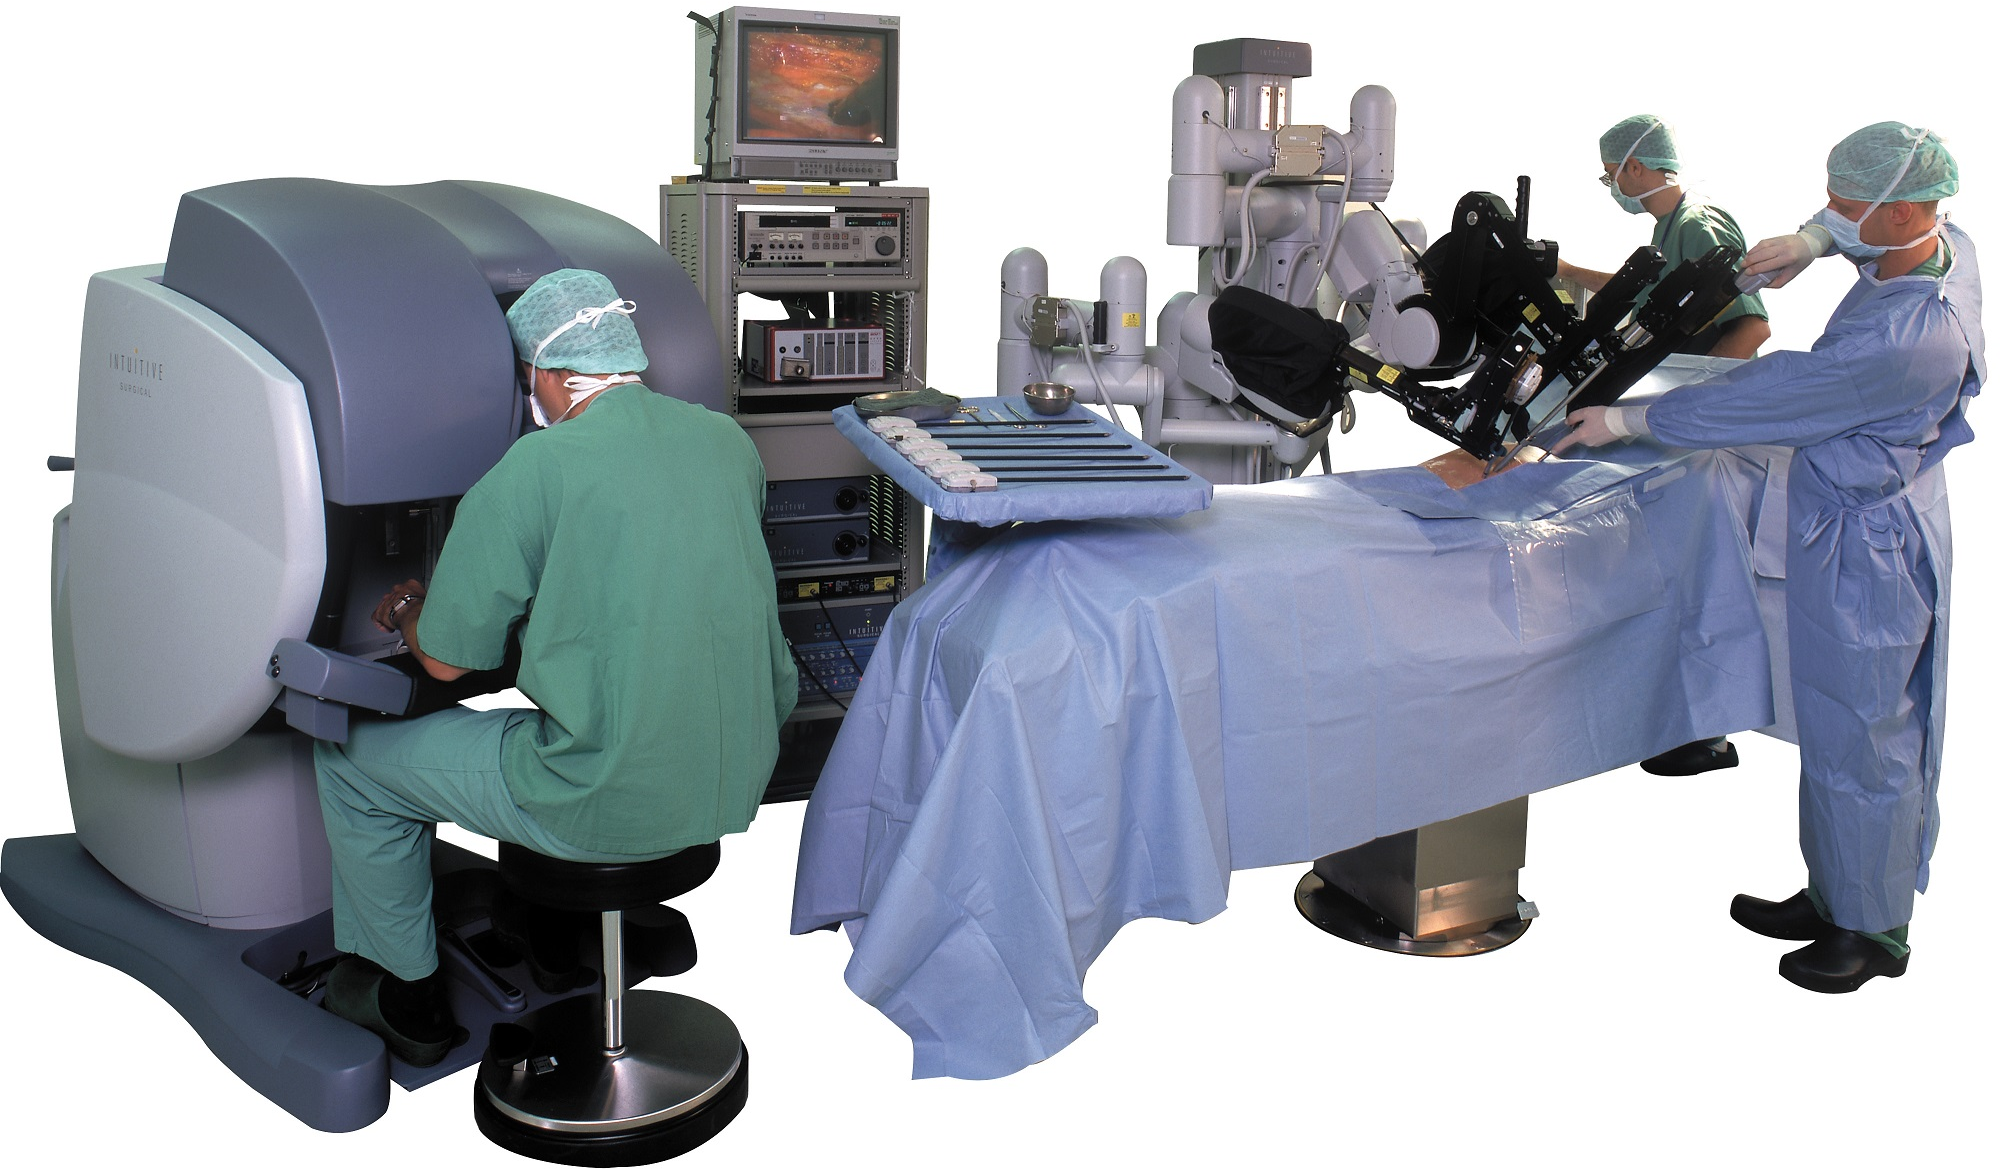
\includegraphics[width=.5\textwidth]{images/fig_01}
}%figues de la page de garde


\def\xxpied{%
%Cycle 05 -- Modélisation mécanique -- Énergétique\\% afin de valider leurs performances.\\
%Chapitre 1 -- \xxactivite%
}

\setcounter{secnumdepth}{5}
%---------------------------------------------------------------------------


\begin{document}
%\chapterimage{png/Fond_Cin}
\input{style/new_pagegarde}
\vspace{5.5cm}
\pagestyle{fancy}
\thispagestyle{plain}


\def\columnseprulecolor{\color{ocre}}
\setlength{\columnseprule}{0.4pt} 

%\ifprof
%\else
\begin{multicols}{2}
%\fi
\section*{Mise en situation}
\ifprof
\else
\fi

L'objet de l'étude est un << siège motorisé >> destiné à des navites de luxe. Cette motorisation permet de rendre le siège plus ergonomique. On s'intéresse en particulier ou basculement avant -- arrière du fauteuil.

\begin{center}
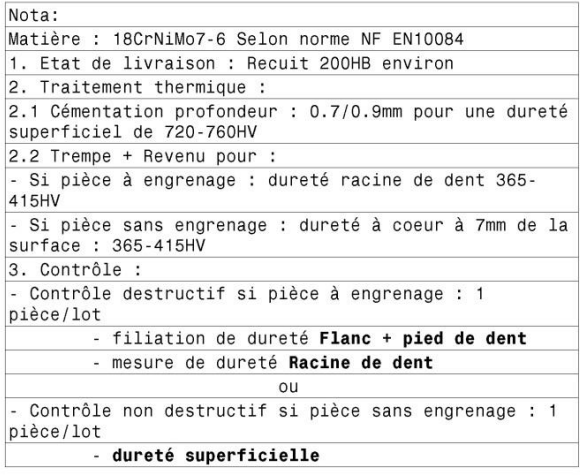
\includegraphics[height=3.5cm]{images/fig_02}
\hspace{1cm}
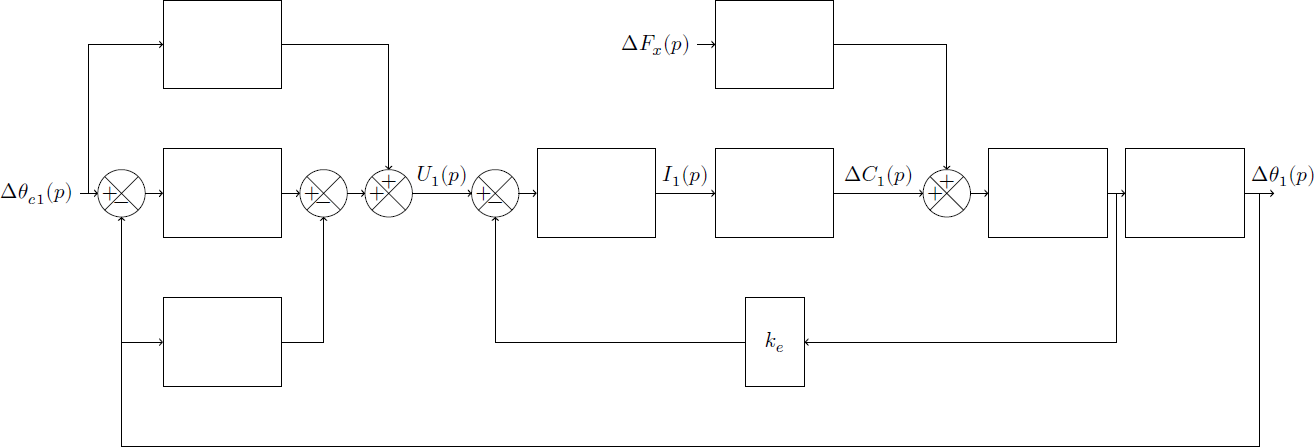
\includegraphics[height=3.5cm]{images/fig_03}
\end{center}

L'ensemble étudié est constitué d'un ensemble fixe (lié au bateau), d'un ensemble pivot, basculant et du support de siège.

\begin{center}
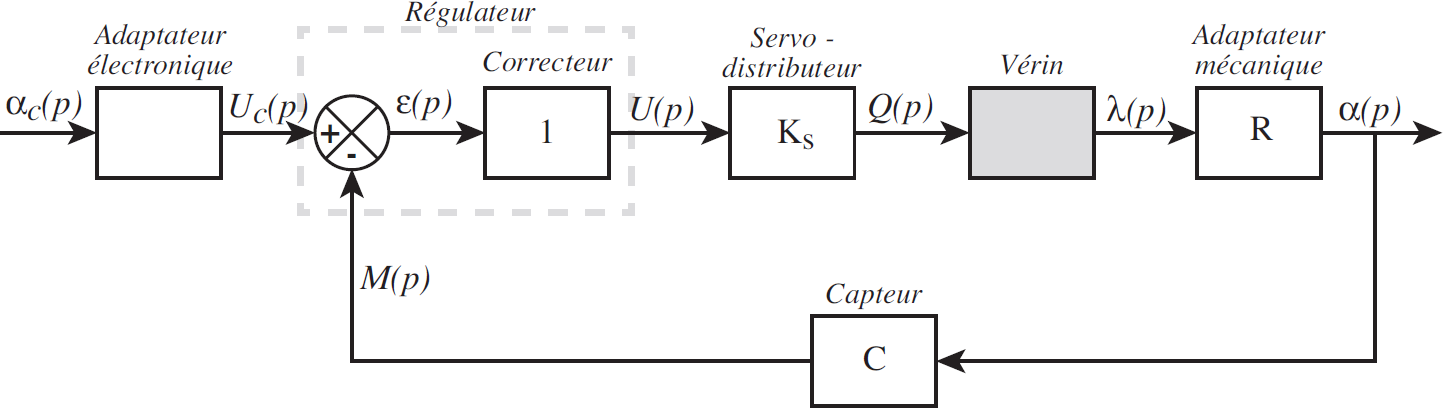
\includegraphics[width=\linewidth]{images/fig_04}
\end{center}

La chappe, objet des questions qui suivent, permet de faire la liaison entre l'ensemble pivot et l'ensemble basculant. 

\subsection*{Analyse des spécifications}
\subparagraph{}\textit{Justifier pourquoi $A$, $B$ et $C$ sont utilisées comme surface de référence ?}

\subparagraph{}\textit{Comment peut-on justifier fonctionnellement l'existence des spécifications suivantes ?}

\begin{center}
\includegraphics[width=.5\linewidth]{images/gps_00}
\end{center}


\subparagraph{}\textit{Analyser les spécifications suivantes.}

\begin{center}
\includegraphics[width=.25\linewidth]{images/gps_01}
\hfill
\includegraphics[width=.3\linewidth]{images/gps_02}
\hfill
\includegraphics[width=.3\linewidth]{images/gps_03}
\end{center}

\subparagraph{}\textit{Quel serait l'effet d'un modificateur au maximum de matière sur l'exigence de localisation ? (exigence du maximum de matière porté sur la tolérance).}


\subsection*{Analyse des procédés de fabrication}

\subparagraph{}\textit{Après avoir proposé un (ou plusieurs) moyens d'obtention du brut, préciser les différents étapes de fabrication de la chape.}

\subparagraph{}\textit{Proposer une gamme de fabrication ainsi que les mises en position associées à chacun des phases.}



\end{multicols}


\begin{center}
{\includegraphics[width=\linewidth]{images/Dessin}}

\rotatebox{270}{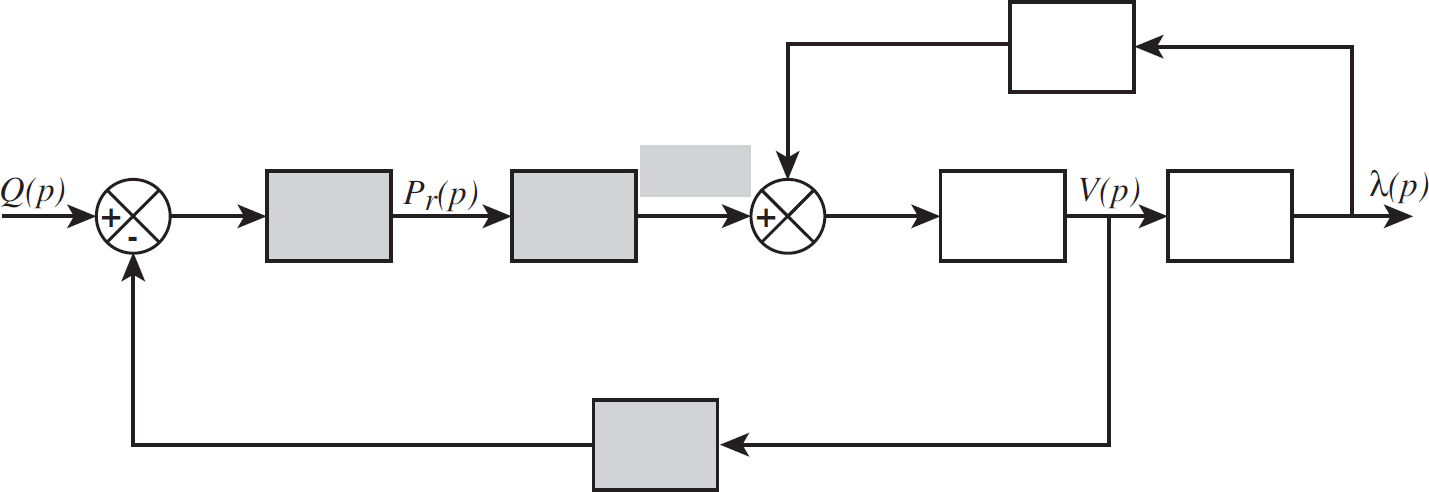
\includegraphics[height=\linewidth]{images/fig_06}}
\end{center}


\end{document}

\subparagraph{}\textit{}
\ifprof
\begin{corrige}~\\
\end{corrige}
\else
\fi




\subparagraph{}\textit{}
\ifprof
\begin{corrige}~\\
\end{corrige}
\else
\fi

\subparagraph{}\textit{}
\ifprof
\begin{corrige}~\\
\end{corrige}
\else
\fi

\subparagraph{}\textit{}
\ifprof
\begin{corrige}~\\
\end{corrige}
\else
\fi

\subparagraph{}\textit{}
\ifprof
\begin{corrige}~\\
\end{corrige}
\else
\fi

\subparagraph{}\textit{}
\ifprof
\begin{corrige}~\\
\end{corrige}
\else
\fi

\subparagraph{}\textit{}
\ifprof
\begin{corrige}~\\
\end{corrige}
\else
\fi
\begin{center}
%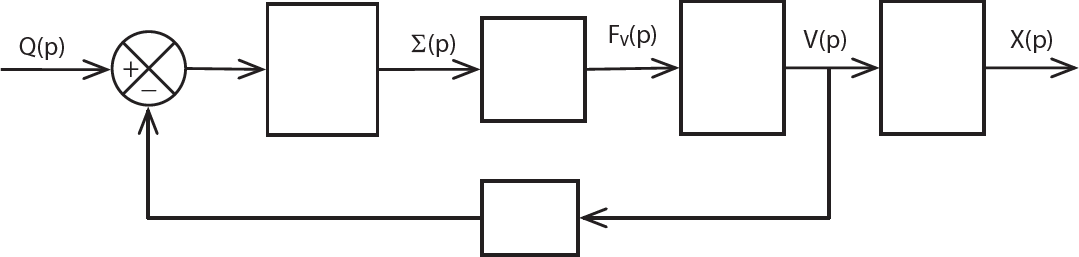
\includegraphics[width=\linewidth]{images/fig_05}
\end{center}
